Разрабатываемый в данном курсовом проекте узел состоит из нескольких логических частей: устройства управления (УУ), трехразрядного регистра режима и непосредственно формирователя импульсной последовательности. Структурная схема приведена на рис. \ref{fig:structure}.\\
Структурная схема многофункционального формирователя импульсной последовательности приведена на рис. \ref{fig:nodestructure}

\begin{figure}
  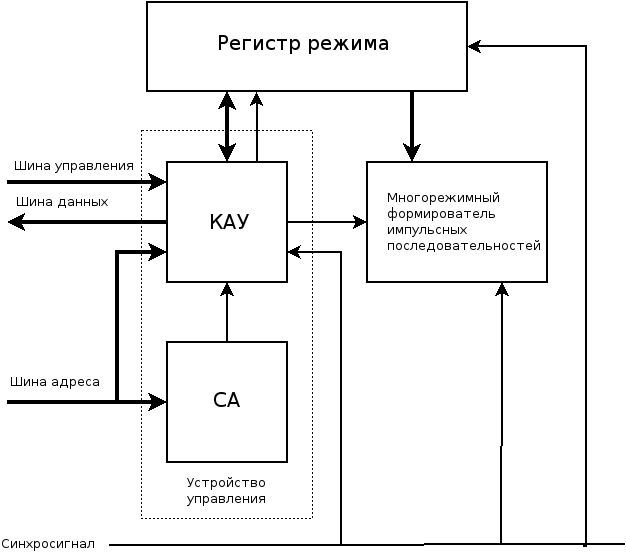
\includegraphics[scale=0.58]{./structure.png}
  \caption{Структура узла. СА - селектор адреса, КАУ - конечный автомат управления.}
  \label{fig:structure}
\end{figure}

\begin{figure}
  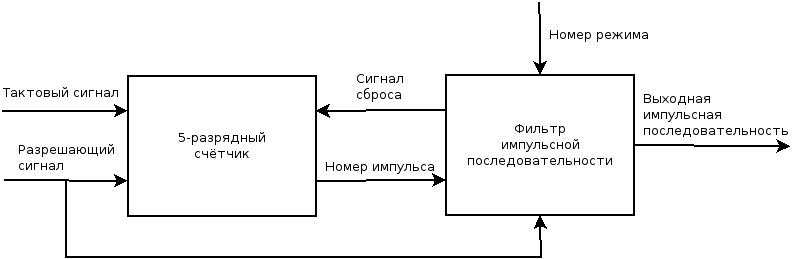
\includegraphics[scale=0.58]{./node-structure.png}
  \caption{Структура многофункционального формирователя импульсной последовательности}
  \label{fig:nodestructure}
\end{figure}

Для корректной работы устройства должны присутствовать:
\begin{itemize}
\item Шина данных (ШД)
\item Шина управления (ШУ)
\item Шина адреса (ША)
\item Тактирующий сигнал
\end{itemize}
\noindent Подробное описание интерфейса разрабатываемого устройства и протокол его работы представлены в разделе <<\nameref{sections:iface}>>

